% Options for packages loaded elsewhere
\PassOptionsToPackage{unicode}{hyperref}
\PassOptionsToPackage{hyphens}{url}
\PassOptionsToPackage{dvipsnames,svgnames,x11names}{xcolor}
%
\documentclass[
  letterpaper,
  DIV=11,
  numbers=noendperiod]{scrartcl}

\usepackage{amsmath,amssymb}
\usepackage{iftex}
\ifPDFTeX
  \usepackage[T1]{fontenc}
  \usepackage[utf8]{inputenc}
  \usepackage{textcomp} % provide euro and other symbols
\else % if luatex or xetex
  \usepackage{unicode-math}
  \defaultfontfeatures{Scale=MatchLowercase}
  \defaultfontfeatures[\rmfamily]{Ligatures=TeX,Scale=1}
\fi
\usepackage{lmodern}
\ifPDFTeX\else  
    % xetex/luatex font selection
\fi
% Use upquote if available, for straight quotes in verbatim environments
\IfFileExists{upquote.sty}{\usepackage{upquote}}{}
\IfFileExists{microtype.sty}{% use microtype if available
  \usepackage[]{microtype}
  \UseMicrotypeSet[protrusion]{basicmath} % disable protrusion for tt fonts
}{}
\makeatletter
\@ifundefined{KOMAClassName}{% if non-KOMA class
  \IfFileExists{parskip.sty}{%
    \usepackage{parskip}
  }{% else
    \setlength{\parindent}{0pt}
    \setlength{\parskip}{6pt plus 2pt minus 1pt}}
}{% if KOMA class
  \KOMAoptions{parskip=half}}
\makeatother
\usepackage{xcolor}
\setlength{\emergencystretch}{3em} % prevent overfull lines
\setcounter{secnumdepth}{5}
% Make \paragraph and \subparagraph free-standing
\ifx\paragraph\undefined\else
  \let\oldparagraph\paragraph
  \renewcommand{\paragraph}[1]{\oldparagraph{#1}\mbox{}}
\fi
\ifx\subparagraph\undefined\else
  \let\oldsubparagraph\subparagraph
  \renewcommand{\subparagraph}[1]{\oldsubparagraph{#1}\mbox{}}
\fi


\providecommand{\tightlist}{%
  \setlength{\itemsep}{0pt}\setlength{\parskip}{0pt}}\usepackage{longtable,booktabs,array}
\usepackage{calc} % for calculating minipage widths
% Correct order of tables after \paragraph or \subparagraph
\usepackage{etoolbox}
\makeatletter
\patchcmd\longtable{\par}{\if@noskipsec\mbox{}\fi\par}{}{}
\makeatother
% Allow footnotes in longtable head/foot
\IfFileExists{footnotehyper.sty}{\usepackage{footnotehyper}}{\usepackage{footnote}}
\makesavenoteenv{longtable}
\usepackage{graphicx}
\makeatletter
\def\maxwidth{\ifdim\Gin@nat@width>\linewidth\linewidth\else\Gin@nat@width\fi}
\def\maxheight{\ifdim\Gin@nat@height>\textheight\textheight\else\Gin@nat@height\fi}
\makeatother
% Scale images if necessary, so that they will not overflow the page
% margins by default, and it is still possible to overwrite the defaults
% using explicit options in \includegraphics[width, height, ...]{}
\setkeys{Gin}{width=\maxwidth,height=\maxheight,keepaspectratio}
% Set default figure placement to htbp
\makeatletter
\def\fps@figure{htbp}
\makeatother
% definitions for citeproc citations
\NewDocumentCommand\citeproctext{}{}
\NewDocumentCommand\citeproc{mm}{%
  \begingroup\def\citeproctext{#2}\cite{#1}\endgroup}
\makeatletter
 % allow citations to break across lines
 \let\@cite@ofmt\@firstofone
 % avoid brackets around text for \cite:
 \def\@biblabel#1{}
 \def\@cite#1#2{{#1\if@tempswa , #2\fi}}
\makeatother
\newlength{\cslhangindent}
\setlength{\cslhangindent}{1.5em}
\newlength{\csllabelwidth}
\setlength{\csllabelwidth}{3em}
\newenvironment{CSLReferences}[2] % #1 hanging-indent, #2 entry-spacing
 {\begin{list}{}{%
  \setlength{\itemindent}{0pt}
  \setlength{\leftmargin}{0pt}
  \setlength{\parsep}{0pt}
  % turn on hanging indent if param 1 is 1
  \ifodd #1
   \setlength{\leftmargin}{\cslhangindent}
   \setlength{\itemindent}{-1\cslhangindent}
  \fi
  % set entry spacing
  \setlength{\itemsep}{#2\baselineskip}}}
 {\end{list}}
\usepackage{calc}
\newcommand{\CSLBlock}[1]{\hfill\break\parbox[t]{\linewidth}{\strut\ignorespaces#1\strut}}
\newcommand{\CSLLeftMargin}[1]{\parbox[t]{\csllabelwidth}{\strut#1\strut}}
\newcommand{\CSLRightInline}[1]{\parbox[t]{\linewidth - \csllabelwidth}{\strut#1\strut}}
\newcommand{\CSLIndent}[1]{\hspace{\cslhangindent}#1}

\KOMAoption{captions}{tableheading}
\makeatletter
\@ifpackageloaded{caption}{}{\usepackage{caption}}
\AtBeginDocument{%
\ifdefined\contentsname
  \renewcommand*\contentsname{Table of contents}
\else
  \newcommand\contentsname{Table of contents}
\fi
\ifdefined\listfigurename
  \renewcommand*\listfigurename{List of Figures}
\else
  \newcommand\listfigurename{List of Figures}
\fi
\ifdefined\listtablename
  \renewcommand*\listtablename{List of Tables}
\else
  \newcommand\listtablename{List of Tables}
\fi
\ifdefined\figurename
  \renewcommand*\figurename{Figure}
\else
  \newcommand\figurename{Figure}
\fi
\ifdefined\tablename
  \renewcommand*\tablename{Table}
\else
  \newcommand\tablename{Table}
\fi
}
\@ifpackageloaded{float}{}{\usepackage{float}}
\floatstyle{ruled}
\@ifundefined{c@chapter}{\newfloat{codelisting}{h}{lop}}{\newfloat{codelisting}{h}{lop}[chapter]}
\floatname{codelisting}{Listing}
\newcommand*\listoflistings{\listof{codelisting}{List of Listings}}
\makeatother
\makeatletter
\makeatother
\makeatletter
\@ifpackageloaded{caption}{}{\usepackage{caption}}
\@ifpackageloaded{subcaption}{}{\usepackage{subcaption}}
\makeatother
\ifLuaTeX
  \usepackage{selnolig}  % disable illegal ligatures
\fi
\usepackage{bookmark}

\IfFileExists{xurl.sty}{\usepackage{xurl}}{} % add URL line breaks if available
\urlstyle{same} % disable monospaced font for URLs
\hypersetup{
  pdftitle={Mini-rotations - Trophic overyielding and infection dynamics},
  pdfauthor={Cole Brookson},
  colorlinks=true,
  linkcolor={blue},
  filecolor={Maroon},
  citecolor={Blue},
  urlcolor={Blue},
  pdfcreator={LaTeX via pandoc}}

\title{Mini-rotations - Trophic overyielding and infection dynamics}
\author{Cole Brookson}
\date{2024-04-05}

\begin{document}
\maketitle
\begin{abstract}
Working through ideas for the mini-rotations project
\end{abstract}

\renewcommand*\contentsname{Table of contents}
{
\hypersetup{linkcolor=}
\setcounter{tocdepth}{3}
\tableofcontents
}
\section{Background}

Previous work has shown that the coexistence of a pair or mixture of
species can reach higher abundance than the species with the highest
carrying capacity (Loreau 2004; Poisot \emph{et al.} 2013). This idea of
``transgressive overyielding'' is the basis for much work on
biodiversity-ecosystem functioning relationships (BEF) (i.e., Schmid
\emph{et al.} 2008). Some research has suggested approaches to linking
this concept to disease dynamics (Johnson \emph{et al.} 2015), however,
few studies have explicitly developed theory to this effect. Noteably
Sieben \emph{et al.} (2022) and others have provided elegant frameworks
for considering competition and coexistence from the perspective of
parasites themselves existing in both between- and within-host
frameworks. However,
\textbf{what effects do infection dynamics have on transgressive overyielding?}
Is it possible that the inclusion of pathogen dynamics into classic
models of competition would change the conditions under which
transgressive overyielding is founded? If so, what is the relation of
the virulence of the infection and the basic reproductive number
\(\mathcal{R_0}\)?

\section{Methods}

We start from the assumption of two species competing, in a
Lotka-Volterra model. We use the form of Abrams (2022, pg. 39), which
includes terms for both inter- and intra-specific competition. We then
have

\begin{equation}
  \label{eqn:simple-lv-1}
  \frac{dN_1}{dt} = N_1(r_1 - \alpha_{11}N_1 - \alpha_{12}N_2)
\end{equation} \begin{equation}
  \label{eqn:simple-lv-2}
  \frac{dN_2}{dt} = N_2(r_2 - \alpha_{21}N_1 - \alpha_{22}N_2)
\end{equation}

The relation to the original generalized Lotka-Volterra model (as
pointed out by Abrams 2022) is that \(\alpha_{ii} = \frac{1}{K_i}\) and
\(\alpha_{ij} = \frac{\alpha_{ij}}{K_i}\).

Further and related, we can imagine one of these species becoming
infected with a generalized pathogen. The closed population of that
species now can be thought of as being described by a standard
compartment model. That is, the number of individuals in \(N_1\) can be
thought of as divided into individuals that are susceptible, \(S_1\),
infected \(I_1\), and recovered \(R_1\) such that

\begin{equation} 
\label{eqn:sum-sir}
  N_1 = S_1 + I_1 + R_1
\end{equation}

Further, we can then think of these dynamics as being described by a
classic \(SIR\) model with the dynamics given by:

\begin{equation}
\label{eqn:basic-sir-s}
  \frac{dS}{dt} = - \beta S I + \delta R 
\end{equation}

\begin{equation}
\label{eqn:basic-sir-i}
  \frac{dI}{dt} = \beta S I - \gamma I 
\end{equation}

\begin{equation}
\label{eqn:basic-sir-r}
  \frac{dR}{dt} = \gamma I - \delta R
\end{equation}

\subsection{Transgressive Overyielding}

To understand how the incorporation of infection dynamics may affect the
conditions under which transgressive overyielding happens, our goals are
to:

\begin{enumerate}
\def\labelenumi{\arabic{enumi})}
\tightlist
\item
  Re-derive an expression for transgressive overyielding from the inter-
  and intra-specific version of the GLV (Eqns \ref{eqn:simple-lv-1}
  \ref{eqn:simple-lv-2})
\item
  Re-state this expression in terms of the infection parameters that
  will affect the inter-specifi competition
\item
  Assess the assumption of non-linear growth on these expressions
\item
\end{enumerate}

\begin{table}[hpt]
\centering
\begin{tabular}{ |m{3cm}||m{10cm}|}
     \hline
     \multicolumn{2}{|c|}{Model Parameters} \\
     \hline
     \textbf{Term} & \textbf{Description} \\
     \hline
     $N_i$ & Abundance of species $i$ \\
     $r_i$ & Growth rate of species $i$ \\
     $\alpha_{ii}$ & Intraspecific competition within species $i$ \\
     $\alpha_{ij}$ & Interspecific competition between species $i$ and $j$ \\
     $S_i$ & Number of susceptible individuals in population $i$ \\
     $I_i$ & Number of infected individuals in population $i$ \\
     $R_i$ & Number of recovered individuals in population $i$ \\
     $\beta$ & Rate at which susceptible individuals become infected \\
     $\delta$ & Rate at which recovered individuals lose their immunity and become susceptible again \\
     $\gamma$ & Rate at which the infected individuals recover from infection \\
     \hline
\end{tabular}
\caption{Parameter values for our model systems}
\label{table:parameters}
\end{table}

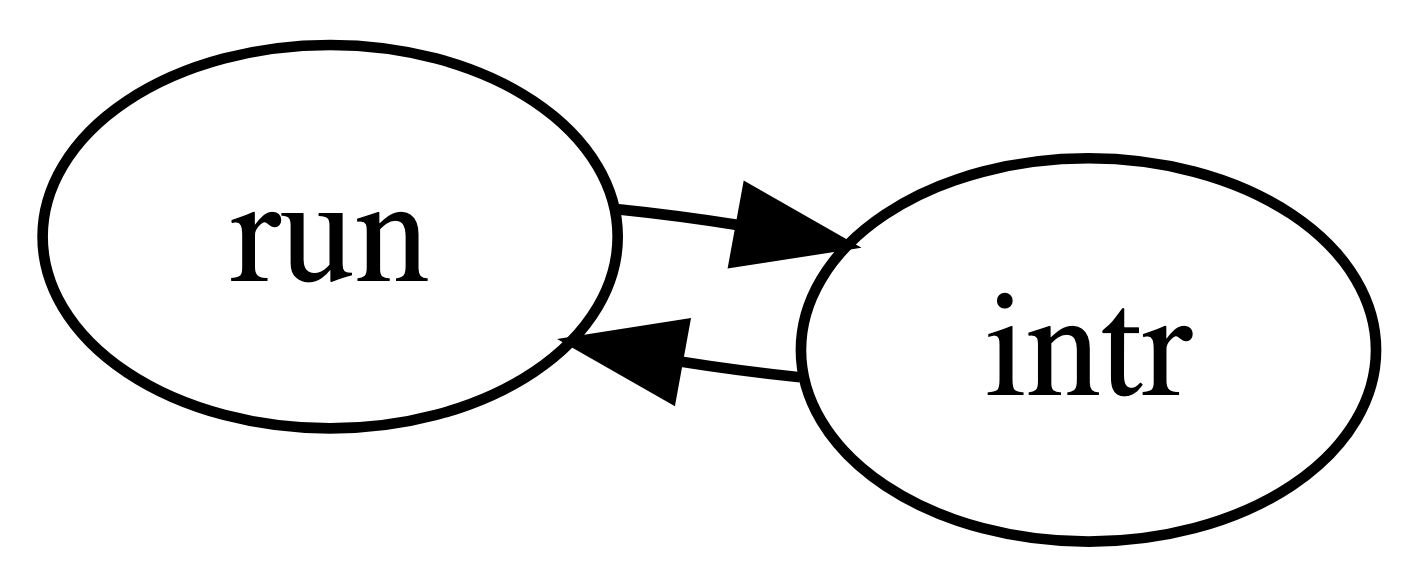
\includegraphics[width=5.5in,height=3.5in]{index_files/figure-latex/dot-figure-1.png}

\section{References}

\textsubscript{Source:
\href{https://colebrookson.github.io/disease-overyield/index.qmd.html}{Article
Notebook}}

\phantomsection\label{refs}
\begin{CSLReferences}{1}{0}
\bibitem[\citeproctext]{ref-abrams_competition_2022}
Abrams, P.A. (2022).
\emph{\href{https://books.google.ca/books?hl=en&lr=&id=fTaFEAAAQBAJ&oi=fnd&pg=PP1&dq=abrams+2022+competition+theory&ots=_cdJwLVcq_&sig=ZUB2hKd4WD_YZsynGVHu114pnJ4}{Competition
theory in ecology}}. Oxford University Press.

\bibitem[\citeproctext]{ref-johnson_frontiers_2015}
Johnson, P.T.J., Ostfeld, R.S. \& Keesing, F. (2015).
\href{https://doi.org/10.1111/ele.12479}{Frontiers in research on
biodiversity and disease}. \emph{Ecology Letters}, 18, 1119--1133.

\bibitem[\citeproctext]{ref-loreau_does_2004}
Loreau, M. (2004).
\href{https://doi.org/10.1111/j.0030-1299.2004.12685.x}{Does functional
redundancy exist?} \emph{Oikos}, 104, 606--611.

\bibitem[\citeproctext]{ref-poisot_trophic_2013}
Poisot, T., Mouquet, N. \& Gravel, D. (2013).
\href{https://doi.org/10.1111/ele.12118}{Trophic complementarity drives
the biodiversity--ecosystem functioning relationship in food webs}.
\emph{Ecology Letters}, 16, 853--861.

\bibitem[\citeproctext]{ref-schmid_biodiversity_2008}
Schmid, B., Hector, A., Saha, P. \& Loreau, M. (2008).
\href{https://academic.oup.com/jpe/article-abstract/1/2/95/989985}{Biodiversity
effects and transgressive overyielding}. \emph{Journal of Plant
Ecology}, 1, 95--102.

\bibitem[\citeproctext]{ref-sieben_quantifying_2022}
Sieben, A.J., Mihaljevic, J.R. \& Shoemaker, L.G. (2022).
\href{https://doi.org/10.1002/ecy.3819}{Quantifying mechanisms of
coexistence in disease ecology}. \emph{Ecology}, 103, e3819.

\end{CSLReferences}



\end{document}
